%!TEX program = xelatex+makeindex+bibtex
\documentclass[final]{scrreprt} %scrreprt of scrartcl
% Include all project wide packages here.
\usepackage{fullpage}
\usepackage{polyglossia}
\setmainlanguage{english}
\usepackage{csquotes}
\usepackage{graphicx}
\usepackage{epstopdf}
\usepackage{pdfpages}
\usepackage{caption}
\usepackage[list=true]{subcaption}
\usepackage{float}
\usepackage{standalone}
\usepackage{import}
\usepackage{tocloft}
\usepackage{wrapfig}
\usepackage{authblk}
\usepackage{array}
\usepackage{booktabs}
\usepackage[toc,page,title,titletoc]{appendix}
\usepackage{xunicode}
\usepackage{fontspec}
\usepackage{pgfplots}
\usepackage{SIunits}
\usepackage{units}
\pgfplotsset{compat=newest}
\pgfplotsset{plot coordinates/math parser=false}
\newlength\figureheight 
\newlength\figurewidth
\usepackage{amsmath}
\usepackage{mathtools}
\usepackage{unicode-math}
\usepackage[
    backend=bibtexu,
	texencoding=utf8,
bibencoding=utf8,
    style=ieee,
    sortlocale=en_US,
    language=auto
]{biblatex}
\usepackage{listings}
\newcommand{\includecode}[3][c]{\lstinputlisting[caption=#2, escapechar=, style=#1]{#3}}
\newcommand{\superscript}[1]{\ensuremath{^{\textrm{#1}}}}
\newcommand{\subscript}[1]{\ensuremath{_{\textrm{#1}}}}


\newcommand{\chapternumber}{\thechapter}
\renewcommand{\appendixname}{Bijlage}
\renewcommand{\appendixtocname}{Bijlagen}
\renewcommand{\appendixpagename}{Bijlagen}

\usepackage[hidelinks]{hyperref} %<--------ALTIJD ALS LAATSTE

\renewcommand{\familydefault}{\sfdefault}

\setmainfont[Ligatures=TeX]{Myriad Pro}
\setmathfont{Asana Math}
\setmonofont{Lucida Console}

\usepackage{titlesec, blindtext, color}
\definecolor{gray75}{gray}{0.75}
\newcommand{\hsp}{\hspace{20pt}}
\titleformat{\chapter}[hang]{\Huge\bfseries}{\chapternumber\hsp\textcolor{gray75}{|}\hsp}{0pt}{\Huge\bfseries}
\renewcommand{\familydefault}{\sfdefault}
\renewcommand{\arraystretch}{1.2}
\setlength\parindent{0pt}

%For code listings
\definecolor{black}{rgb}{0,0,0}
\definecolor{browntags}{rgb}{0.65,0.1,0.1}
\definecolor{bluestrings}{rgb}{0,0,1}
\definecolor{graycomments}{rgb}{0.4,0.4,0.4}
\definecolor{redkeywords}{rgb}{1,0,0}
\definecolor{bluekeywords}{rgb}{0.13,0.13,0.8}
\definecolor{greencomments}{rgb}{0,0.5,0}
\definecolor{redstrings}{rgb}{0.9,0,0}
\definecolor{purpleidentifiers}{rgb}{0.01,0,0.01}


\lstdefinestyle{csharp}{
language=[Sharp]C,
showspaces=false,
showtabs=false,
breaklines=true,
showstringspaces=false,
breakatwhitespace=true,
escapeinside={(*@}{@*)},
columns=fullflexible,
commentstyle=\color{greencomments},
keywordstyle=\color{bluekeywords}\bfseries,
stringstyle=\color{redstrings},
identifierstyle=\color{purpleidentifiers},
basicstyle=\ttfamily\small}

\lstdefinestyle{c}{
language=C,
showspaces=false,
showtabs=false,
breaklines=true,
showstringspaces=false,
breakatwhitespace=true,
escapeinside={(*@}{@*)},
columns=fullflexible,
commentstyle=\color{greencomments},
keywordstyle=\color{bluekeywords}\bfseries,
stringstyle=\color{redstrings},
identifierstyle=\color{purpleidentifiers},
}

\lstdefinestyle{matlab}{
language=Matlab,
showspaces=false,
showtabs=false,
breaklines=true,
showstringspaces=false,
breakatwhitespace=true,
escapeinside={(*@}{@*)},
columns=fullflexible,
commentstyle=\color{greencomments},
keywordstyle=\color{bluekeywords}\bfseries,
stringstyle=\color{redstrings},
identifierstyle=\color{purpleidentifiers}
}

\lstdefinestyle{vhdl}{
language=VHDL,
showspaces=false,
showtabs=false,
breaklines=true,
showstringspaces=false,
breakatwhitespace=true,
escapeinside={(*@}{@*)},
columns=fullflexible,
commentstyle=\color{greencomments},
keywordstyle=\color{bluekeywords}\bfseries,
stringstyle=\color{redstrings},
identifierstyle=\color{purpleidentifiers}
}

\lstdefinestyle{xaml}{
language=XML,
showspaces=false,
showtabs=false,
breaklines=true,
showstringspaces=false,
breakatwhitespace=true,
escapeinside={(*@}{@*)},
columns=fullflexible,
commentstyle=\color{greencomments},
keywordstyle=\color{redkeywords},
stringstyle=\color{bluestrings},
tagstyle=\color{browntags},
morestring=[b]",
  morecomment=[s]{<?}{?>},
  morekeywords={xmlns,version,typex:AsyncRecords,x:Arguments,x:Boolean,x:Byte,x:Char,x:Class,x:ClassAttributes,x:ClassModifier,x:Code,x:ConnectionId,x:Decimal,x:Double,x:FactoryMethod,x:FieldModifier,x:Int16,x:Int32,x:Int64,x:Key,x:Members,x:Name,x:Object,x:Property,x:Shared,x:Single,x:String,x:Subclass,x:SynchronousMode,x:TimeSpan,x:TypeArguments,x:Uid,x:Uri,x:XData,Grid.Column,Grid.ColumnSpan,Click,ClipToBounds,Content,DropDownOpened,FontSize,Foreground,Header,Height,HorizontalAlignment,HorizontalContentAlignment,IsCancel,IsDefault,IsEnabled,IsSelected,Margin,MinHeight,MinWidth,Padding,SnapsToDevicePixels,Target,TextWrapping,Title,VerticalAlignment,VerticalContentAlignment,Width,WindowStartupLocation,Binding,Mode,OneWay,xmlns:x}
}

%defaults
\lstset{
basicstyle=\ttfamily\small,
extendedchars=false,
numbers=left,
numberstyle=\ttfamily\tiny,
stepnumber=1,
tabsize=4,
numbersep=5pt
}
\addbibresource{../../library/bibliography.bib}
\title{Module 1 - Report}
\author{Sander {van Dijk} \and Erwin {de Haan}}
\begin{document}

\chapter{Assignment 1}
The designed DC-DC converter is displayed in Figure \ref{fig:DC-AC} and \ref{fig:AC-DC}, splitted in the DC-AC and AC-DC part, respectively.

\begin{figure}[h]
	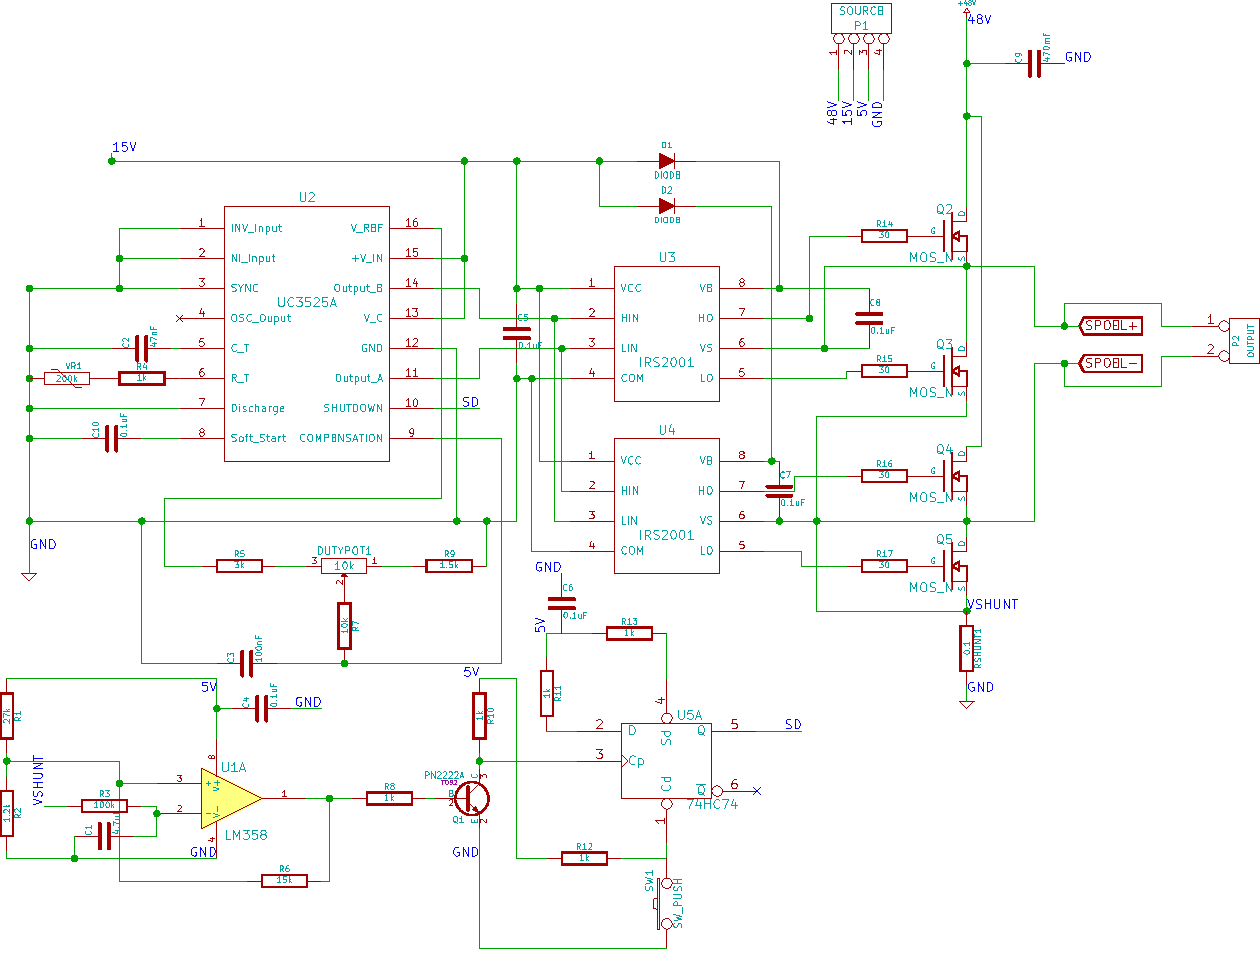
\includegraphics[width=\linewidth]{resources/DC-AC-rc.pdf}
	\caption{DC-AC subcircuit}
	\label{fig:DC-AC}
\end{figure}

\begin{figure}[h]
	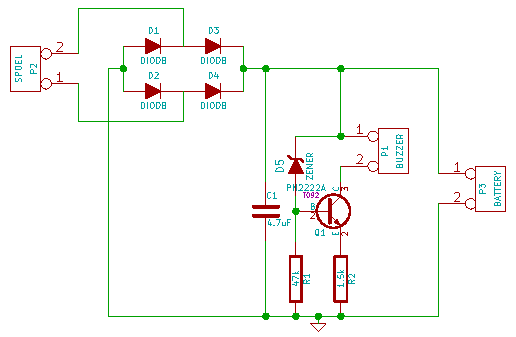
\includegraphics[width=\linewidth]{resources/AC-DC-rc.pdf}
	\caption{AC-DC subcircuit}
	\label{fig:AC-DC}
\end{figure}

For the NMOS transistor used in Figure \ref{fig:DC-AC} we used the IPP028N08N3G (OptiMOS 3) transistor instead of the IPP50CN10N (OptiMOS 2).
We had two reasons for this decision.
First, the drain-source on-state resistance was approximally ten times lower on the OptiMOS 3, causing the transistor to generate less heat and gain better efficiency.
Secondly, by looking at the current-voltage characteristics per frequency (\cite{OptiMOS2} \emph{:3 Safe operating area} and \cite{OptiMOS3} \emph{:3 Safe operating area}) we found out that the OptiMOS 3 performs better at higher frequencies than the OptiMOS 2.
\\ \\
We also had to choose the diodes used on the secondary side of the tranformer. The diodes will form a full bridge rectifier, which in combination with a capacitor, will form a AC-DC converter.
The candidates are the SB540 (datasheet: \cite{SB540}) and the SF61 (datasheet: \cite{SF61}).
The forward voltage of the two diodes differ, the SB540's is lower. This is favorable since there will be more voltage left on the output terminals.
On the other hand, the SF61 has a much lower reverse current. Lower reverse current makes the diode more ideal, since it sould only conduct when the current is in forward direction.
We chose the SF61 since we thought the reverse current would be more important.
\\ \\
After soldering the inverter and rectifier we tested the two parts.
Figure \ref{fig:AandB} displays the voltage on the output-A and output-B of the UC3525a, which are the oscillating opposites of each other.
This oscillating pair drives the transistor H-bridge, powering the primary coil.
The secondary coil will generate a voltage from this primary coil's voltage, which is displayed in Figure \ref{fig:AC_sec}.
This voltage is rectified using the full bridge rectifier and a small capacitor, it is turned into a DC-voltage as shown in Figure \ref{fig:DC_out}.

\begin{figure}[h]
	\begin{center}
		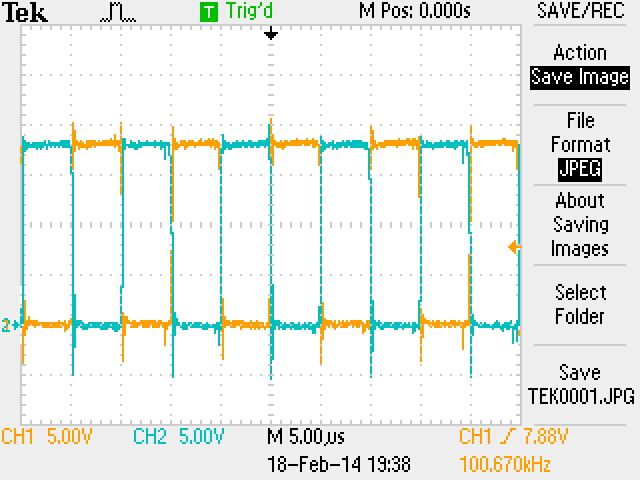
\includegraphics[width=\linewidth/2]{resources/AandB-rc.jpg}
	\end{center}
	\caption{Voltages of nodes A and B on the inverter (UC3525a's outputs)}
	\label{fig:AandB}
\end{figure}

\begin{figure}[h]
	\begin{center}
		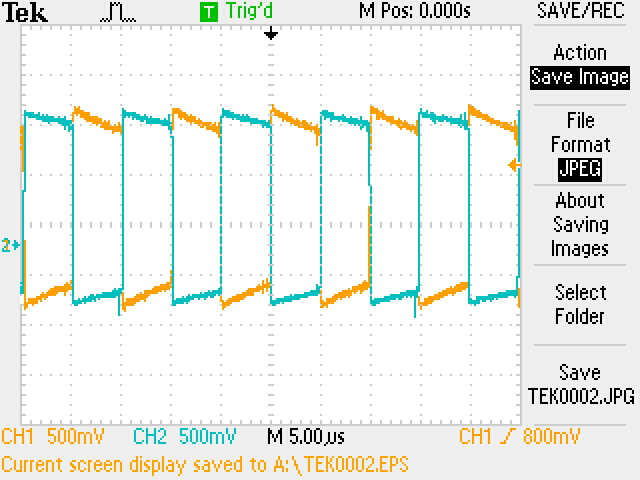
\includegraphics[width=\linewidth/2]{resources/AC_sec-rc.jpg}
	\end{center}
	\caption{Transformed voltage on secondary coils}
	\label{fig:AC_sec}
\end{figure}

\begin{figure}[h]
	\begin{center}
		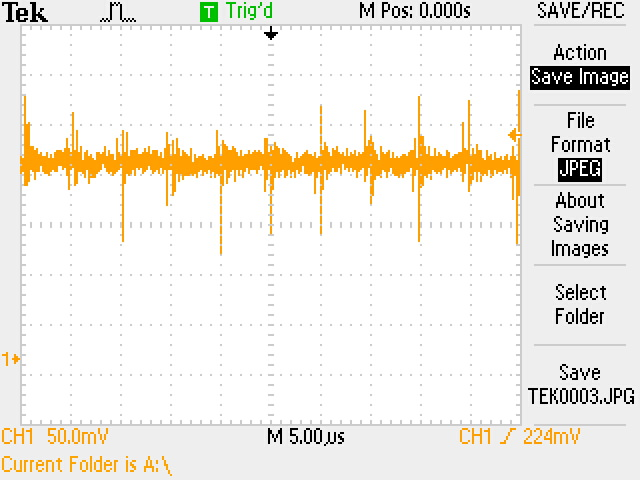
\includegraphics[width=\linewidth/2]{resources/DC_out-rc.jpg}
	\end{center}
	\caption{Output DC voltage}
	\label{fig:DC_out}
\end{figure}

Additionally, we designed a PCB for our design. The multiple layers and silk screen can be found in Figure \ref{fig:PCBcopperTop},  \ref{fig:PCBcopperBottom} and  \ref{fig:PCBcomponents}.

\begin{figure}[h]
	\begin{center}
		\includegraphics[width=\linewidth/2]{resources/DC-AC-F_CU-rc.pdf}
	\end{center}
	\caption{AC-DC PCB front copper layer}
	\label{fig:PCBcopperTop}
\end{figure}

\begin{figure}[h]
	\begin{center}
		\includegraphics[width=\linewidth/2]{resources/DC-AC-B_CU-rc.pdf}
	\end{center}
	\caption{AC-DC PCB bottom copper layer}
	\label{fig:PCBcopperBottom}
\end{figure}

\begin{figure}[h]
	\begin{center}
		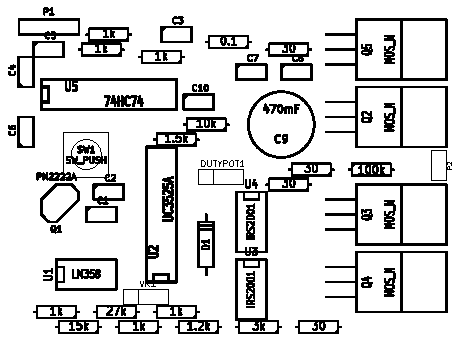
\includegraphics[width=\linewidth/2]{resources/DC-AC-F_SilkS-rc.pdf}
	\end{center}
	\caption{AC-DC PCB silk screen}
	\label{fig:PCBcomponents}
\end{figure}

\end{document}